\lab{Algorithms}{Bayesian Updates}{Bayesian Updates}
\objective{Understand the basic principles of computing a posterior distribution from a prior and data.}
\bf{Dependencies:} emph{Difference between Frequentist and Bayesian paradigms, distributions (Bernoulli, Binomial, Beta, Dirichlet)}\\

All of us are Bayesians, whether we would like to admit it or not. Each of us subconsciously computes probabilities of different outcomes every day. At any given point in time, we have a belief (a \emph{prior}) of how probable any given outcome is, though we may not be able to quantize it. If it occurs or not (our data), we update our belief accordingly (once again, subconsciously). Essentially, this updated belief is called our \emph{posterior}.

As mathematicians and statisticians, we would like to quantify this notion, and it all follows from Bayes Rule:
\begin{equation*}
\mathbb{P}(A | B) = \frac{\mathbb{P}(B | A)\mathbb{P}(A)}{\mathbb{P}(B)}
\end{equation*}

Let us suppose we are going to run a medical trial on a given treatment, where we consider each sample to be a Bernoulli random variable, i.e. success or failure, with parameter $\theta$. Recall that the parameter of a Bernoulli distribution, $\theta$, is the probability of success for a sample.  Note that the sum of $n$ Bernoulli($\theta$) random variables is itself a random variable from a Binomial distribution with parameters $n$ and $\theta$, the same parameter for probability of success. The frequentist approach is to suppose there is no prior knowledge about the chance of success of the treatment. However, we often have some prior knowledge about similar treatments which we can carry over, giving us a \emph{prior} on our parameter $\theta$. This prior essentially relates our belief about the true, unknown value of $\theta$, including its expected value, variance, etc.

Let us suppose that our prior is a beta distribution over $\theta$ with parameters $\alpha$ and $\beta$, i.e. 
\begin{equation*}
\mathbb{P}(\theta) = \frac{\theta^{\alpha - 1}(1 - \theta)^{\beta - 1}}{B(\alpha,\beta)}
\end{equation*}
where $B(\alpha,\beta)$ is the Beta function, such that 
\begin{equation*}
\int_0^1 \theta^{\alpha - 1}(1 - \theta)^{\beta - 1} d\theta = B(\alpha,\beta) = \frac{\Gamma(\alpha)\Gamma(\beta)}{\Gamma(\alpha +\beta)}
\end{equation*}

 Given a sequence of successes or failures $\mathbf{y} = y_{1},\cdots,y_{n}$, where there are $\sum_{i=1}^n y_i = n_{1}$ successes and $(n - \sum_{i=1}^n y_i) = n_{2}$ failures, we can compute our \emph{posterior} distribution of $\theta$, given the data $\mathbf{y}$, as follows:

\begin{align*}
\mathbb{P}(\theta | \mathbf{y}) & = \frac{\mathbb{P}(\mathbf{y} | \theta)\mathbb{P}(\theta)}{\mathbb{P}(\mathbf{y})} \\
& = \frac{\mathbb{P}(\mathbf{y} | \theta)\mathbb{P}(\theta)}{\int_{0}^{1} \mathbb{P}(\mathbf{y} | \theta)\mathbb{P}(\theta) d\theta} \\
& = \frac{{n_{1} + n_{2} \choose n_{1}} \theta^{n_{1}}(1-\theta)^{n_{2}} \frac{\theta^{\alpha - 1}(1 - \theta)^{\beta - 1}}{B(\alpha,\beta)}}{\int_{0}^{1} {n_{1} + n_{2} \choose n_{1}} \theta^{n_{1}}(1-\theta)^{n_{2}} \frac{\theta^{\alpha - 1}(1 - \theta)^{\beta - 1}}{B(\alpha,\beta)} d\theta} \\
& = \frac{ \theta^{n_{1} + \alpha - 1}(1-\theta)^{n_{2} + \beta - 1}}{\int_{0}^{1} \theta^{n_{1} + \alpha - 1}(1-\theta)^{n_{2} + \beta - 1} d\theta} \\
& = \frac{\frac{1}{B(n_{1} + \alpha - 1, n_{2} + \beta - 1)}}{\frac{1}{B(n_{1} + \alpha - 1, n_{2} + \beta - 1)}} \frac{ \theta^{n_{1} + \alpha - 1}(1-\theta)^{n_{2} + \beta - 1}}{\int_{0}^{1} \theta^{n_{1} + \alpha - 1}(1-\theta)^{n_{2} + \beta - 1} d\theta} \\
& = \frac{ \theta^{n_{1} + \alpha - 1}(1-\theta)^{n_{2} + \beta - 1}}{B(n_{1} + \alpha - 1, n_{2} + \beta - 1)}
\end{align*}

This is simply the density of the Beta distribution over $\theta$ with parameters $\alpha + n_{1} - 1$ and $\beta + n_{2} - 1$. Notice that both the prior and posterior are Beta distributions. When the prior and posterior distributions are from the same family, we call the prior ``conjugate'' to the distribution of the data. 

Python has the Beta density built in. Given parameters $\alpha$ and $\beta$, we can evaluate and plot the density for many values of $\theta$:

\begin{lstlisting}
>>> import numpy as np
>>> import matplotlib.pyplot as plt
>>> from scipy.stats import beta
>>> a = 8
>>> b = 2
>>> x = np.arange(0, 1.01, .01)
>>> y = beta.pdf(x, a, b)
>>> plt.plot(x, y)
>>> plt.show()
\end{lstlisting}

\begin{figure}[h]
\begin{center}
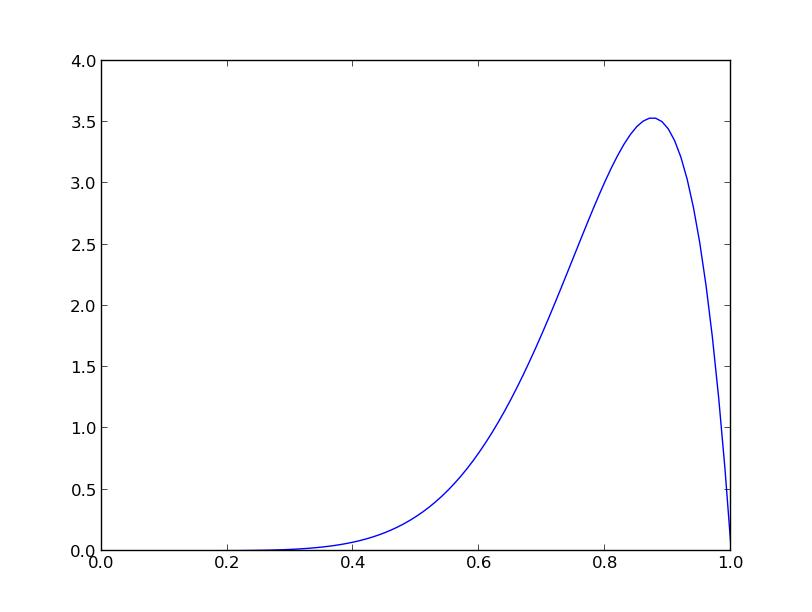
\includegraphics[height=1.5in]{beta.jpeg}
\end{center}
\caption{Beta density function with parameters $\alpha = 8$ and $\beta = 2$.}
\end{figure}

\begin{problem}
Write a function that accepts a data set of i.i.d. Bernoulli random variables and parameters $\alpha$ and $\beta$ (for a beta prior over $\theta$), and which plots the posterior distribution of $\theta$. Test it on the data in the file \emph{trial.csv}, picking your own prior parameters $\alpha$ and $\beta$. How did your belief about the treatment success rate ($\theta$) change?
\end{problem}

Let's now suppose that we run a fruit stand, selling apples, bananas, mangos, oranges, and watermelons. We assume that when a person comes and buys fruit, he selects one piece of fruit. This can be modeled as a draw from a categorical distribution with parameter $\theta$. The Categorical distribution is a discrete probability distribution over the $k$ possible events, the multiple-event version of the Bernoulli distribution.  The combination/mutual occurence of $n$ Categorical variables is called a Multinomial variable (the multiple-event version )with probability mass function
$$$$

five kinds of fruit, also a Multinomial distribution with $n=1$). Thus $\theta$ is a vector of length five, with non-negative entries summing to $1$, each entry being the probability of selecting the corresponding fruit.

We don't know what $\theta$ is, but we have some prior belief of the populace's fruit preferences, which we represent as a Dirichlet prior over $\theta$ with parameter vector $\alpha$, that is, $$\mathbb{P}(\theta) = \frac{1}{B(\alpha)} \prod_{i=1}^{5} \theta_{i}^{\alpha_{i} - 1}$$ where $B(\alpha)$ is the multinomial Beta function, $$B(\alpha) = \frac{\prod_{i=1}^{5} \Gamma(\alpha_{i})}{\Gamma(\sum_{i=1}^{5} \alpha_{i})}.$$ Given a sequence of fruit selections $\mathbf{y} = y_{1}, \cdots, y_{n}$ from $n$ people, where each $$y_{i} \in \{\text{Apple, Banana, Mango, Orange, Watermelon}\},$$ we let 
\begin{align*}
n_{1} & = |\{1 \leq i \leq n | y_{i} = \text{Apple}\}| \\
n_{2} & = |\{1 \leq i \leq n | y_{i} = \text{Banana}\}| \\
\vdots & = \; \; \; \; \; \; \; \; \; \; \; \; \; \; \; \; \; \; \vdots \\
n_{5} & = |\{1 \leq i \leq n | y_{i} = \text{Watermelon}\}|
\end{align*}

Given this new data of people's purchases, we can compute our posterior distribution of $\theta$ as follows:
\begin{align*}
\mathbb{P}(\theta | \mathbf{y}) & = \frac{\mathbb{P}(\mathbf{y} | \theta) \mathbb{P}(\theta)}{\int \mathbb{P}(\mathbf{y} | \theta) \mathbb{P}(\theta) d\theta} \\
& = \frac{\prod_{i=1}^{5} \theta_{i}^{n_{i}} \frac{1}{B(\alpha)} \prod_{i=1}^{5} \theta_{i}^{\alpha_{i}-1}}{\int \cdots \int \prod_{i=1}^{5} \theta_{i}^{n_{i}} \frac{1}{B(\alpha)} \prod_{i=1}^{5} \theta_{i}^{\alpha_{i}-1} d\theta_{1}\cdots d\theta_{5}} \\
& = \frac{\prod_{i=1}^{5} \theta_{i}^{n_{i} + \alpha_{i} - 1}}{\int \cdots \int \prod_{i=1}^{5} \theta_{i}^{n_{i} + \alpha_{i} - 1} d\theta_{1} \cdots d\theta_{5}} \\
& = \frac{\frac{1}{B(n + \alpha)}}{\frac{1}{B(n+\alpha)}} \frac{\prod_{i=1}^{5} \theta_{i}^{n_{i} + \alpha_{i} - 1}}{\int \cdots \int \prod_{i=1}^{5} \theta_{i}^{n_{i} + \alpha_{i} - 1} d\theta_{1} \cdots d\theta_{5}} \\
& = \frac{\prod_{i=1}^{5} \theta_{i}^{n_{i} + \alpha_{i} - 1}}{B(n + \alpha)}
\end{align*}
where $$n = \left( \begin{array}{ccccc} n_{1} & n_{2} & n_{3} & n_{4} & n_{5} \end{array} \right).$$

\begin{problem}
Write a multinomial Beta function that accepts a vector of nonnegative reals of arbitrary length.
\end{problem}

\begin{problem}
Write a function that accepts a data set of i.i.d. draws from a Categorical($\theta$) distribution, a parameter vector $\alpha$ for the Dirichlet prior over $\theta$, and a set of unique categories (in our example, fruits). Have this function return the Dirichlet parameter for the posterior distribution of $\theta$. Test it with the data set in the file \emph{fruit.csv} and a prior $$\alpha = \left( \begin{array}{ccccc} 5 & 3 & 4 & 2 & 1 \end{array} \right).$$
\end{problem}

Now suppose that we have a set of exam scores $\mathbf{y} = y_{1}, \cdots, y_{n}$ from the university's calculus final. Historically, we know how people have scored on the exam, giving us information to make a prior on the distribution of scores. We also know that the scores should be Normally distributed, $X_i \sim N(\mu,\sigma^2)$, $i=1,...,n$. Here we are encountering something new: a prior for a distribution with two parameters instead of one. What we do is place a prior on each parameter. We let $\mu \sim N(\mu_{0}, \sigma_{0}^{2})$ and $\sigma^{2} \sim IG(\alpha, \beta)$ be priors for our mean and variance, respectively, where $IG$ is the Inverse Gamma distribution, with probability density function:

$$\mathbb{P}(\sigma^{2}) = \frac{\beta^{\alpha}}{\Gamma(\alpha)}(\sigma^{2})^{-\alpha - 1}e^{-\frac{\beta}{\sigma^{2}}}\text{; } \alpha,\beta,\sigma^2 >0.$$

\begin{problem}
Write your own function to compute an Inverse Gamma probability density function given parameters $\alpha$ and $\beta$. It should be able to compute the density at an array of values. Call it \emph{invgammapdf}.
\end{problem}

Let's look at how to plot each of these prior distributions:

\begin{lstlisting}
>>> from scipy.stats import norm
>>> mu_0 = 74.
>>> sigma2_0 = 25.
>>> alpha = 2.
>>> beta = 25.
>>> x = np.arange(0, 100.1, step=0.1)
>>> y = norm.pdf(x, loc=mu_0, scale=5)
>>> plt.plot(x, y)
>>> plt.show()
>>> x = np.arange(0.1, 100.1, step=0.1)
>>> y = invgammapdf(x, alpha=alpha, beta=beta)
>>> plt.plot(x, y)
>>> plt.show()
\end{lstlisting}

\begin{figure}[h]
\centering
\begin{subfigure}[b]{.49\textwidth}
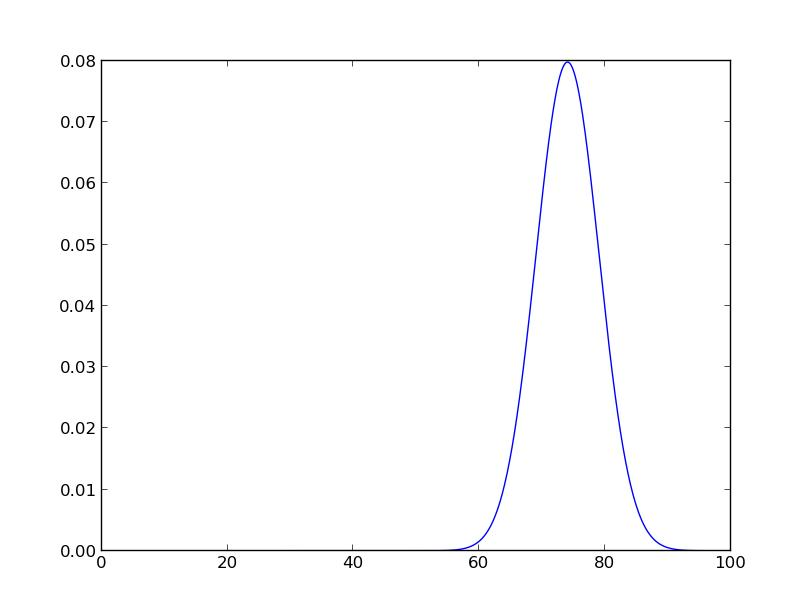
\includegraphics[width=\textwidth]{mean_prior.jpeg}
\caption{Prior distribution for $\mu$.}
\end{subfigure}
\begin{subfigure}[b]{.49\textwidth}
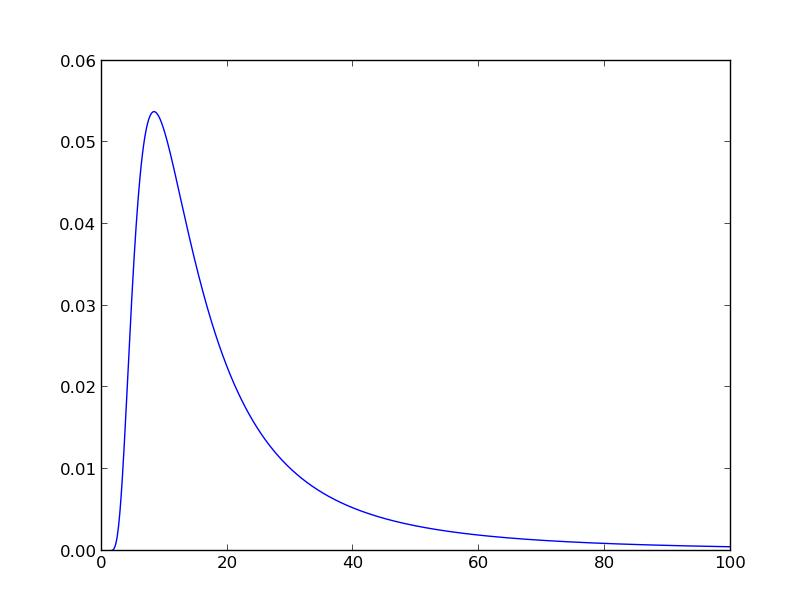
\includegraphics[width=\textwidth]{variance_prior.jpeg}
\caption{Prior distribution for $\sigma^{2}$.}
\end{subfigure}
\caption{Plots of prior distributions}
\end{figure}

For now, let us suppose that we can assume a true value for one of the two parameters. Supposing first that we know the true variance $\sigma^{2}$ for the distribution of scores, the posterior distribution of $\mu$ given the data $\mathbf{y}$ is
$$\mu | \mathbf{y} \sim N\left(\frac{\frac{\mu_{0}\sigma^{2}}{n} + \overline{\mathbf{y}}\sigma_{0}^{2}}{\frac{\sigma^{2}}{n} + \sigma_{0}^{2}}, \left(\frac{n}{\sigma^{2}} + \frac{1}{\sigma_{0}^{2}}\right)^{-1}\right),$$
where $\overline{\mathbf{y}}$ is the average of the data points in $\mathbf{y}$. Now, if we know the true mean $\mu$ for the score distribution, the posterior distribution of $\sigma^{2}$ given the data $\mathbf{y}$ is $$\sigma^{2} | \mathbf{y} \sim IG \left(\alpha + \frac{n}{2}, \beta + \frac{\sum_{i=1}^{n} (y_{i} - \mu)^{2}}{2}\right).$$

\begin{problem}
Write a function that accepts a data set of real numbers, a prior ($\mu_{0}$ and $\sigma_{0}^{2}$) for the mean $\mu$ of a normal distribution, and the true variance $\sigma^{2}$ of the distribution, and returns the updated posterior parameters for $\mu$. Test it on the data in the file \emph{examscores.csv} with prior $\mu_{0} = 74, \sigma_{0}^{2} = 25$ and true variance $\sigma^{2} = 36$. Plot your posterior distribution for $\mu$.
\end{problem}

\begin{problem}
Write a function that accepts a dataset of real numbers, a prior ($\alpha$ and $\beta$) for the variance $\sigma^{2}$ of a normal distribution, and the true mean $\mu$ of the distribution, and returns the updated posterior parameters for $\sigma^{2}$. Test it on the data in the file \emph{examscores.csv} with prior $\alpha=2, \beta = 25$ and true mean $\mu = 62$. Plot your posterior distribution for $\sigma^{2}$.
\end{problem}